\scanpage{48}
\diagram{\begin{tikzcd}[ampersand replacement=\&, column sep=small]0\arrow[r,no head]\&P'\arrow[r,no head]\&P\arrow[r,no head]\&P''\arrow[r,no head]\&\unsure{0|\bullet}\&Q\end{tikzcd}}
\margin{\figure{\begin{tikzpicture}\fill (0,0) ellipse (.03 and .015);\end{tikzpicture}}}
\deleted{$\unsure{nP''=0}$}
\[\text{\inserted{a)}}\quad nQ=Q\qquad\text{b)\raisebox{-.7ex}{\begin{tikzpicture}[x=.04cm,y=.04cm]\draw (0,0) ellipse (1 and .65);\end{tikzpicture}}}\quad {}_nP\mathbin{-}P''\quad\text{épimorphisme}\]
Toute biextension \inserted{\begin{tabular}[b]{@{}c@{}}$E$\\[-.6ex]\begin{tikzpicture}[x=.08cm,y=.08cm]\draw (0,2)--(1,0)--(2,2);\end{tikzpicture}\end{tabular}} de $P\times Q$ \deleted{\unsure{définit}} par $G$ définit

a) Une biextension \inserted{\begin{tabular}[b]{@{}c@{}}$E'$\\[-.6ex]\begin{tikzpicture}[x=.08cm,y=.08cm]\draw (0,2)--(1,0)--(2,2);\end{tikzpicture}\end{tabular}} de $P'\times Q$ par $G$

d'où un accouplement
\diagram{\begin{tikzcd}[ampersand replacement=\&]{}_nP'\times{}_nQ\arrow[r,"E'(n)"]\&G\end{tikzcd}}
\margin{\begingroup
\setbox0=\hbox{%
  \let\ScanOverlaySavedSout\sout
  \let\sout\relax
  \deleted{%
    \let\sout\ScanOverlaySavedSout
    \parbox{.36\linewidth}{\unsure{c)|Si} La \deleted{\unsure{suite}} $0\mathbin{-}P'\mathbin{-}P\mathbin{-}P''\mathbin{-}0$ est \unsure{splittée} \deleted{\unsure{ou}} \uline{ou} elle est
\[\deleted{\operatorname{Hom}(P\otimes Q,G)\longrightarrow\operatorname{Hom}(P'\otimes Q,G)}\]
\uline{loc.} \uline{\unsure{splittée}} et
\[\underline{\operatorname{Hom}}(P'\otimes Q,G)=0\]}}}
\dimen0=\wd0 \advance\dimen0 by 8pt
\dimen2=\ht0 \advance\dimen2 by \dp0 \advance\dimen2 by 8pt
\leavevmode\rlap{\raisebox{\dimexpr-\dp0-4pt\relax}{%
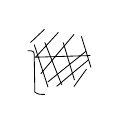
\begin{tikzpicture}[x={\dimexpr\dimen0/578\relax},y={\dimexpr-\dimen2/326\relax},line width=.3pt]
\path[use as bounding box] (0,0) rectangle (578,326);
\draw (0,109)..controls (45,108) and (55,112)..(55,130)--(60,305)..controls (85,316) and (116,318)..(144,316);
\draw (24,70)--(141,8) (68,139)--(258,22) (110,218)--(389,32) (169,257)--(491,111) (243,278)--(513,151) (388,279)--(494,196);
\draw (55,80)--(171,282) (144,70)--(285,270) (298,70)--(393,248) (451,41)--(531,188);
\draw (56,140)--(526,132);
\end{tikzpicture}}}%
\kern4pt\box0\kern4pt\endgroup}

b) Une biextension de ${}_nP\times Q$ par $G$, i.e. un accouplement
\diagram{\begin{tikzcd}[ampersand replacement=\&]{}_nP\times{}_nQ\arrow[r,"\varphi"]\&G\end{tikzcd}}

\deleted{Avec \unsure{le|la|les}} Ces deux $(E',\varphi)$ satisfont la condition que
\[\varphi|({}_nP'\times{}_nQ)=E'(n)\]

\margin{\figure{\begin{tikzpicture}\fill (0,.45) circle (.02);\fill (0,0) circle (.03);\end{tikzpicture}}}
Un hom de biextensions $E_1\longrightarrow E_2$ définit un hom $(E'_1,\varphi_1)\mathbin{-}(E'_2,\varphi_2)$, \begingroup
\setbox0=\hbox{i.e. \inserted{(déf)} un hom de}
\dimen0=\wd0 \advance\dimen0 by 8pt
\dimen2=\ht0 \advance\dimen2 by \dp0 \advance\dimen2 by 8pt
\leavevmode\rlap{\raisebox{\dimexpr-\dp0-4pt\relax}{%
\begin{tikzpicture}[x={\dimexpr\dimen0/365\relax},y={\dimexpr-\dimen2/92\relax},line width=.3pt]
\path[use as bounding box] (0,0) rectangle (365,92);
\draw (117,68)..controls (126,38) and (182,43)..(203,21);
\end{tikzpicture}}}%
\kern4pt\box0\kern4pt\endgroup biextensions $u:E'_1\unsure{\longrightarrow|\mathbin{-}}E'_2$\raisebox{-1ex}{\begin{tikzpicture}[x=.04cm,y=.04cm]\draw (0,0)..controls (-.12,-.4) and (-.1,-.8)..(0,-1);\end{tikzpicture}}, tel que $\varphi\sim$

\uline{Je dis que le foncteur} $E\longmapsto(E',\varphi)$ \uline{est une équiv. de catégories}.

\begingroup
\setbox0=\hbox{%
  \let\ScanOverlaySavedSout\sout
  \let\sout\relax
  \deleted{%
    \let\sout\ScanOverlaySavedSout
    \parbox{.95\linewidth}{\deleted{a) \uline{\unsure{pl. fid.}}}\quad\deleted{b) \unsure{pl. fid.|pl fd}}
\[
\deleted{\text{i.e.}\quad\text{a)}\quad\operatorname{Hom}(P\otimes Q,\unsure{G|C})\xrightarrow{\sim}\operatorname{Hom}(P'\otimes Q,G)}
\]
\[\deleted{\text{b)}\quad E_1\simeq E_2\quad\text{ssi}\quad(E'_1,\varphi_1)\simeq(E'_2,\varphi_{\unsure{2|1}})}\]
\uline{Pl. fidèle} signifie aussi que $E\vdash E|(P',Q)$ est pl. fd, \unsure{i.e.|ou} encore, \deleted{\unsure{que|par}} par la suite exacte, \unsure{que|pour}
\[
\unsure{\text{et}|(*)}\quad\operatorname{Hom}(P''\otimes Q,\unsure{G|C})=0,\qquad
\inserted{(**)}\quad\operatorname{Hom}(P\otimes Q,\unsure{G|C})\longrightarrow\operatorname{Hom}(P'\otimes Q,\unsure{G|C})\quad\uuline{\text{surj.}}
\]
\deleted{\unsure{Ce qui est} \illegible{1} \unsure{ainsi}}
\deleted{\inserted{$(***)$} si $\unsure{E_1,E_2}$ tel que $\unsure{(E'_1,\varphi_1)|(E',\varphi)}$ $\unsure{\simeq}\ \unsure{1}$ \unsure{alors} $\unsure{E_1\simeq E_2|E_1\sim E_2}$}
\inserted{Si $E$ est tel que $E'\simeq1$, $\varphi=0$, alors $E\simeq1$}

La première assertion résulte de a) et b) qui impliquent $P''\otimes Q=0$, la deuxième résulte de c) [dans la deuxième alternative de c) les deux mbs de $(**)$ sont nuls!]:

\deleted{\uline{\unsure{Ess. surj}}.} \unsure{Pour|Par} $(***)$, on note que si $E'=0$, Alors par la suite ex.\unsure{te|de} $E$ est déterminé par un élément de $\operatorname{Ext}(P''\otimes^{\unsure{L}}Q,\unsure{G|C})$, \unsure{or|à} ceci équivaut : un élément de $\operatorname{Hom}(P''\otimes_{\unsure{-|1}}Q,G)$, on \unsure{donne|trouve} que c'est ce qui définit \unsure{$\varphi$, on|$\varphi_1=0$} gagne.}}}
\dimen0=\wd0 \advance\dimen0 by 8pt
\dimen2=\ht0 \advance\dimen2 by \dp0 \advance\dimen2 by 8pt
\leavevmode\rlap{\raisebox{\dimexpr-\dp0-4pt\relax}{%
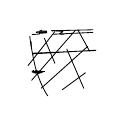
\begin{tikzpicture}[x={\dimexpr\dimen0/1476\relax},y={\dimexpr-\dimen2/1080\relax},line width=.3pt]
\path[use as bounding box] (0,0) rectangle (1476,1080);
\draw (6,597)--(584,60) (83,827)--(1029,36) (288,951)--(1289,292) (736,976)--(1240,706);
\draw (45,131)..controls (58,254) and (150,596)..(177,651)..controls (237,805) and (357,1001)..(432,1071);
\draw (72,215)--(78,289)--(65,263);
\draw (357,163)--(584,561) (1075,34)--(1330,373) (836,332)--(1204,954);
\draw (94,412)--(1465,353) (94,401)--(1465,358);
\draw (548,48)--(1402,33) (546,103)--(1404,74);
\draw (176,67)--(410,62) (176,74)--(410,68) (238,90)--(415,80);
\draw (262,51)..controls (279,35) and (309,39)..(291,51)--(248,55)--(403,54)..controls (411,57) and (414,62)..(408,70);
\draw (89,109)--(266,98);
\draw (531,58)..controls (504,46) and (520,37)..(540,45)--(748,59)..controls (781,62) and (700,78)..(688,91)..controls (670,104) and (725,109)..(785,104);
\draw (91,697)--(367,686);
\draw (90,688)--(123,673)--(119,699)--(162,679)--(147,705)--(197,681)--(180,709)--(231,685)--(212,712)--(259,690)--(244,714)--(290,689)--(279,708)--(329,694);
\end{tikzpicture}}}%
\kern4pt\box0\kern4pt\endgroup

\uline{Corollaire} 1 Supposons, pour un \begingroup
\setbox0=\hbox{$\mathbb{P}$ de \unsure{nbs|nb} premiers}
\dimen0=\wd0 \advance\dimen0 by 8pt
\dimen2=\ht0 \advance\dimen2 by \dp0 \advance\dimen2 by 8pt
\leavevmode\rlap{\raisebox{\dimexpr-\dp0-4pt\relax}{%
\begin{tikzpicture}[x={\dimexpr\dimen0/665\relax},y={\dimexpr-\dimen2/65\relax},line width=.3pt]
\path[use as bounding box] (0,0) rectangle (665,65);
\draw (179,9)--(215,52);
\end{tikzpicture}}}%
\kern4pt\box0\kern4pt\endgroup que
\[\left(\varinjlim_{\substack{n\\\text{\unsure{composé|à support}}\ \mathbb{P}}}{}_nP\right)\longrightarrow P''\quad\text{surjectif},\qquad\text{et que}\quad p\in\mathbb{P}\Longrightarrow pQ=Q.\]
Alors on a une équivalence $E\vdash(E',\varphi)$, \unsure{i.e.|où} $E$ est \unsure{une|un}
\margin{47}
